\documentclass[border=10pt]{standalone}
\usepackage{tikz}
\usepackage[utf8]{inputenc}
\usepackage[T1]{fontenc}
\usetikzlibrary{patterns,arrows.meta,decorations.pathreplacing}

\begin{document}

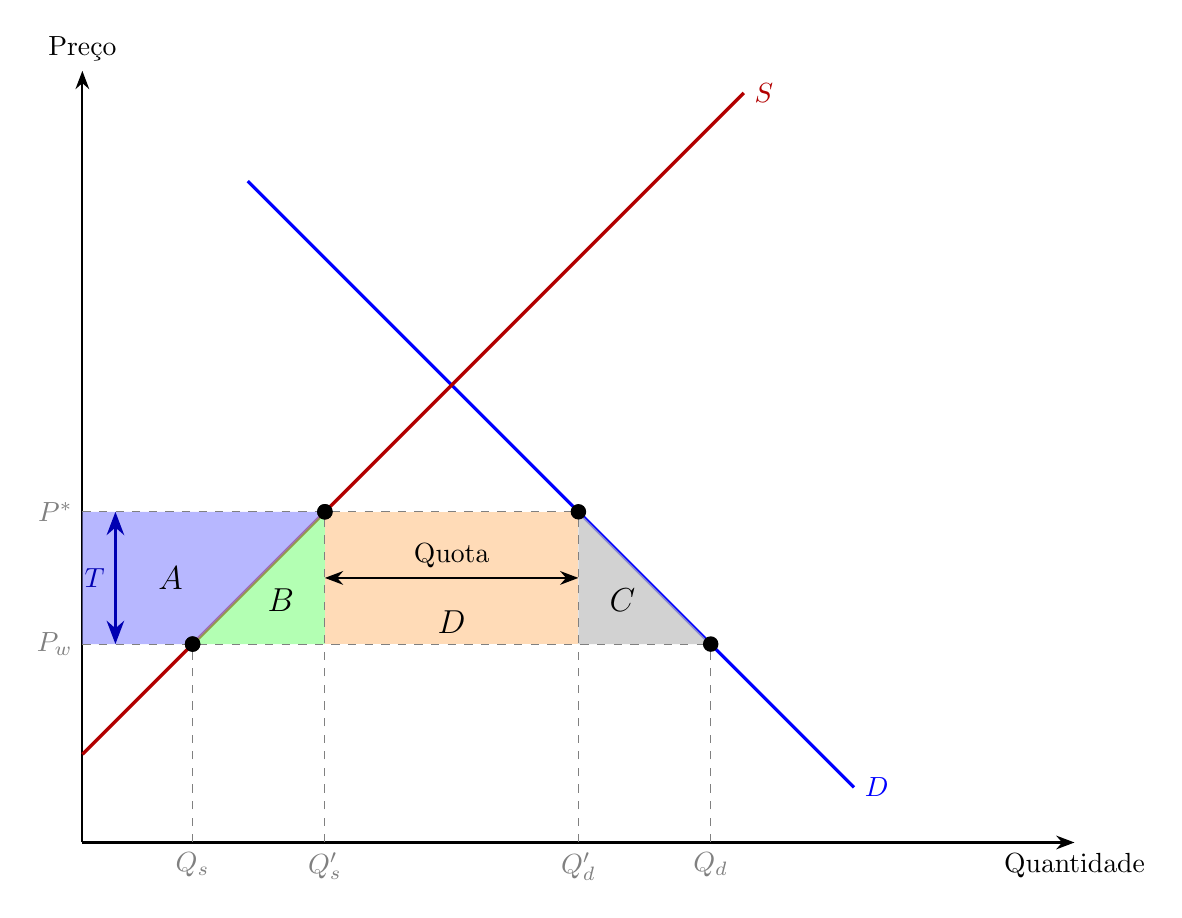
\begin{tikzpicture}[scale=1.4, >=Stealth]
    
    % Eixos
    \draw[thick,->] (0,0) -- (9,0) node[below] {Quantidade};
    \draw[thick,->] (0,0) -- (0,7) node[above] {Preço};
    
    % Curvas de oferta e demanda - mais verticais
    \draw[blue, very thick, domain=1.5:7] plot (\x, {7.5 - 1.0*\x}) node[right] {$D$};
    \draw[red!70!black, very thick, domain=0:6] plot (\x, {0.8 + 1.0*\x}) node[right] {$S$};
    
    % Coordenadas importantes
    % Novas curvas: D: y = 7.5 - 1.0*x, S: y = 0.8 + 1.0*x
    \def\Pw{1.8}        % Preço mundial (mais baixo)
    \def\Pt{3.0}        % Preço com tarifa/quota (mais baixo)
    % Qs: 1.8 = 0.8 + 1.0*x => x = 1.0
    \def\Qs{1.0}        % Qs - oferta doméstica a Pw
    % Qs': 3.0 = 0.8 + 1.0*x => x = 2.2
    \def\Qsp{2.2}       % Qs' - oferta doméstica a P*
    % Qd: 1.8 = 7.5 - 1.0*x => x = 5.7
    \def\Qd{5.7}        % Qd - demanda a Pw
    % Qd': 3.0 = 7.5 - 1.0*x => x = 4.5
    \def\Qdp{4.5}       % Qd' - demanda a P*
    
    % Área A (ganho dos produtores) - entre Pw e P*, à esquerda da curva S
    % Polígono: (0, Pw), (0, P*), (Qs', P*), seguir curva S até (Qs, Pw)
    % S em Qs=1.0: y = 0.8 + 1.0*1.0 = 1.8 (Pw)
    % S em Qs'=2.2: y = 0.8 + 1.0*2.2 = 3.0 (P*)
    \fill[blue!40, opacity=0.7] (0,\Pw) -- (0,\Pt) -- (\Qsp,\Pt) -- plot[domain=\Qsp:\Qs] (\x, {0.8 + 1.0*\x}) -- (\Qs,\Pw) -- cycle;
    
    % Área B (perda de peso morto da produção) - triângulo entre Pw e P*, Qs e Qs', abaixo da curva S
    % Polígono: (Qs, Pw), (Qs', Pw), (Qs', P*), seguir curva S de volta até (Qs, Pw)
    % S em Qs=1.0: y = 0.8 + 1.0*1.0 = 1.8 (Pw)
    % S em Qs'=2.2: y = 0.8 + 1.0*2.2 = 3.0 (P*)
    \fill[green!50, opacity=0.6] (\Qs,\Pw) -- (\Qsp,\Pw) -- (\Qsp,\Pt) -- plot[domain=\Qsp:\Qs] (\x, {0.8 + 1.0*\x}) -- cycle;
    
    % Área D (receita da quota/tarifa - retângulo entre P* e Pw, Qs' e Qd')
    \fill[orange!40, opacity=0.7] (\Qsp,\Pw) rectangle (\Qdp,\Pt);
    
    % Área C (perda de peso morto do consumo)
    \fill[gray!50, opacity=0.7] (\Qdp,\Pt) -- (\Qd,\Pw) -- (\Qdp,\Pw) -- cycle;
    
    % Linhas tracejadas horizontais
    \draw[dashed, gray] (0,\Pt) node[left] {$P^*$} -- (\Qdp,\Pt);
    \draw[dashed, gray] (0,\Pw) node[left] {$P_w$} -- (\Qd,\Pw);
    
    % Linhas tracejadas verticais
    \draw[dashed, gray] (\Qs,0) node[below] {$Q_s$} -- (\Qs,\Pw);
    \draw[dashed, gray] (\Qsp,0) node[below] {$Q'_s$} -- (\Qsp,\Pt);
    \draw[dashed, gray] (\Qdp,0) node[below] {$Q'_d$} -- (\Qdp,\Pt);
    \draw[dashed, gray] (\Qd,0) node[below] {$Q_d$} -- (\Qd,\Pw);
    
    % Seta indicando T (tarifa)
    \draw[<->, very thick, blue!70!black] (0.3,\Pw) -- (0.3,\Pt) node[midway, left] {$T$};
    
    % Setas e texto "Quota" dentro do retângulo D
    \draw[<->, thick] (\Qsp,{(\Pw+\Pt)/2}) -- (\Qdp,{(\Pw+\Pt)/2}) node[midway, above] {Quota};
    
    % Rótulos das áreas
    % Área A: polígono à esquerda da curva S, entre Pw e P*
    % Centro aproximado: considerando eixo Y e curva S
    \node at (0.8, 2.4) {\large $A$};
    % Área B: triângulo com vértices aproximados (Qs, Pw), (Qs', Pw), (Qs', P*)
    % Centróide: ((1.0+2.2+2.2)/3, (1.8+1.8+3.0)/3) = (1.8, 2.2)
    \node at (1.8, 2.2) {\large $B$};
    % Área C: triângulo (Qd', P*), (Qd, Pw), (Qd', Pw)
    % Centróide: ((4.5+5.7+4.5)/3, (3.0+1.8+1.8)/3) = (4.9, 2.2)
    \node at (4.9, 2.2) {\large $C$};
    % Área D: retângulo (Qs', Pw) a (Qd', P*)
    % Centro: ((2.2+4.5)/2, (1.8+3.0)/2) = (3.35, 2.4)
    % Movido para baixo para evitar sobreposição com setas
    \node at (3.35, 2.0) {\large $D$};
    
    % Pontos importantes
    \fill (\Qs,\Pw) circle (2pt);
    \fill (\Qsp,\Pt) circle (2pt);
    \fill (\Qdp,\Pt) circle (2pt);
    \fill (\Qd,\Pw) circle (2pt);
    
    % Pontos de interseção das curvas com os preços
    \fill (\Qs,{0.8 + 1.0*\Qs}) circle (2pt);
    \fill (\Qsp,{0.8 + 1.0*\Qsp}) circle (2pt);
    
\end{tikzpicture}

\end{document}
